\section{参数与输入扰动}
\label{sec:odesens-parameter-input}

初值只是数据的一部分。方程里的系数是估计出来的，外部输入有噪声，方程本身也只是对真实规律的近似。这些改变看上去性质各异，其实都改变了同一件事：曲线每一时刻的变化率。它们都可以写成积分方程中的残差，于是定理~\ref{thm:odesens-basic-estimate}一次解决全部情形。

\paragraph{统一成积分方程中的扰动}
设$\bm{x}$解$\dot{\bm{x}}=\bm{f}(t,\bm{x})$，$\bm{y}$解被改变的方程$\dot{\bm{y}}=\tilde{\bm{f}}(t,\bm{y})$。把$\bm{y}$的方程改写成
\[
 \dot{\bm{y}}=\bm{f}(t,\bm{y})+\bm{r}(t),\qquad
 \bm{r}(t)=\tilde{\bm{f}}(t,\bm{y}(t))-\bm{f}(t,\bm{y}(t)).
\]
这里$\bm{r}$沿着曲线$\bm{y}$取值，是一个只依赖时间的函数。图~\ref{fig:odesens-perturbation-sources}列出了各种改变的去向。

\begin{BookInlineFigure}
  \centering
  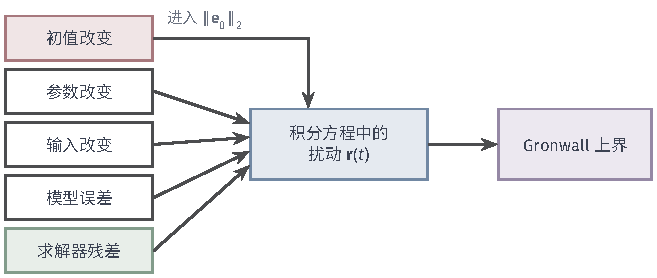
\includegraphics[width=111.2mm]{figures/06-differential-equations/01-ordinary-differential-equations/tikz/odesens-perturbation-sources/figure.pdf}
  \caption{各类改变进入同一个估计的路径。初值改变进入起点的差，参数、输入、模型与数值计算的改变都写成随时间变化的残差$\bm{r}(t)$，再由式~\eqref{eq:odesens-basic-estimate}转成曲线距离的上界。}
  \label{fig:odesens-perturbation-sources}
\end{BookInlineFigure}

\begin{theorem}[右端扰动下的比较]
\label{thm:odesens-perturbation}
设$\bm{x},\bm{y}:[t_0,T]\to\bm{K}$绝对连续，分别几乎处处满足$\dot{\bm{x}}=\bm{f}(t,\bm{x})$、$\dot{\bm{y}}=\tilde{\bm{f}}(t,\bm{y})$。设$\bm{f}$在$\bm{K}$上满足式~\eqref{eq:odesens-lipschitz}，$L$可积，且残差
\begin{equation}
 \varepsilon(t)=\bigl\lVert\tilde{\bm{f}}(t,\bm{y}(t))-\bm{f}(t,\bm{y}(t))\bigr\rVert_2
 \label{eq:odesens-residual}
\end{equation}
可积。记$\Lambda(t)=\int_{t_0}^{t}L$。则
\begin{equation}
 \lVert\bm{y}(t)-\bm{x}(t)\rVert_2\leq\mathrm{e}^{\Lambda(t)}\lVert\bm{y}_0-\bm{x}_0\rVert_2+\int_{t_0}^{t}\mathrm{e}^{\Lambda(t)-\Lambda(s)}\varepsilon(s)\,\mathrm{d}s.
 \label{eq:odesens-perturbation-bound}
\end{equation}
\end{theorem}

\begin{proof}
取定理前定义的残差$\bm{r}$，则$\lVert\bm{r}\rVert_2=\varepsilon$，$\bm{y}$满足定理~\ref{thm:odesens-basic-estimate}中带残差的方程。代入式~\eqref{eq:odesens-basic-estimate}即得结论。
\end{proof}

定理只要求$\bm{f}$有Lipschitz常数，对$\tilde{\bm{f}}$没有要求，它甚至可以不连续。这在比较真实系统与简化模型时有用：真实规律$\tilde{\bm{f}}$往往未知也不光滑，只要它的轨迹$\bm{y}$存在，并且能估计模型在这条轨迹上的误差$\varepsilon$。定理的$\bm{y}$仍须事先知道留在$\bm{K}$内；$\bm{f}$与$\tilde{\bm{f}}$足够接近时，第~\ref{sec:odesens-initial}节的管道论证可以保证这一点。

\paragraph{参数改变}
设右端依赖参数$\bm{\theta}$，且关于参数满足
\[
 \lVert\bm{f}(t,\bm{a},\tilde{\bm{\theta}})-\bm{f}(t,\bm{a},\bm{\theta})\rVert_2\leq\ell(t)\lVert\tilde{\bm{\theta}}-\bm{\theta}\rVert_2,
\]
其中$\ell$可积。此时残差不超过$\ell(s)$乘以参数差的范数，初值相同时，式~\eqref{eq:odesens-perturbation-bound}化为
\begin{equation}
 \lVert\bm{y}(t)-\bm{x}(t)\rVert_2\leq\lVert\tilde{\bm{\theta}}-\bm{\theta}\rVert_2\int_{t_0}^{t}\mathrm{e}^{\Lambda(t)-\Lambda(s)}\ell(s)\,\mathrm{d}s.
 \label{eq:odesens-parameter-bound}
\end{equation}
所以解在紧时间段上Lipschitz依赖参数，前提与初值情形相同。

\begin{example}[增长率改变$20\%$]
\label{ex:odesens-parameter-bound}
考虑$\dot{x}=\theta x(1-x)$，$x_0=1/4$，比较$\theta=1$与$\tilde{\theta}=1.2$在$T=\ln3$时的值。解都留在$\bm{K}=[0,1]$内，$\theta=1$的右端关于$x$的导数是$1-2x$，取$L=1$。残差是
\[
 r(s)=0.2\,y(s)\bigl(1-y(s)\bigr),\qquad \lvert r(s)\rvert\leq0.05.
\]

用$\lvert r\rvert\leq0.05$的粗略界，由式~\eqref{eq:odesens-constant-estimate}得到
\[
 \lvert y(T)-x(T)\rvert\leq0.05\,(\mathrm{e}^{T}-1)=0.1.
\]
若把残差沿$y$的实际值代入式~\eqref{eq:odesens-perturbation-bound}，数值积分得到上界$0.0901$。真实差是$y(T)-x(T)=0.5547-0.5=0.0547$。
\end{example}

图~\ref{fig:odesens-parameter-bound}显示了$[0,3]$上的情况。上界在$t$较大时远离真实差，原因和图~\ref{fig:odesens-bound-vs-true}(c)相同：$L=1$对应$x$靠近$0$时的增长，而$x$靠近$1$时真实的放大率是负的。

\begin{BookInlineFigure}
  \centering
  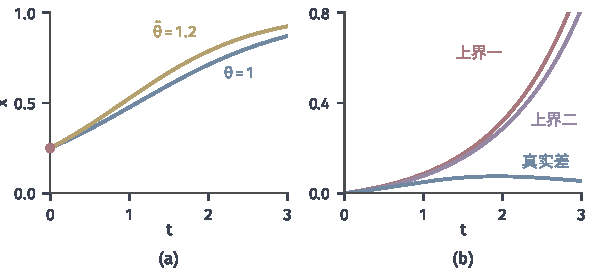
\includegraphics[width=100mm]{figures/06-differential-equations/01-ordinary-differential-equations/matplotlib/odesens-parameter-bound/figure.pdf}
  \caption{参数改变对$\dot{x}=\theta x(1-x)$的影响，$x_0=1/4$。(a)$\theta=1$（蓝）与$\tilde\theta=1.2$（黄）的解。(b)两解的真实差（蓝）、用$\lvert r\rvert\leq0.05$的上界一（红）和用残差实际值的上界二（紫）。}
  \label{fig:odesens-parameter-bound}
\end{BookInlineFigure}

\paragraph{输入改变}
设方程是$\dot{\bm{x}}=\bm{f}(t,\bm{x},\bm{g}(t))$，$\bm{g}$是可测的外部输入。应该用什么范数衡量输入的差？答案取决于右端怎样依赖输入，我们看三种情形。

设右端关于输入值Lipschitz，
\[
 \lVert\bm{f}(t,\bm{a},\tilde{\bm{g}})-\bm{f}(t,\bm{a},\bm{g})\rVert_2\leq\ell(t)\lVert\tilde{\bm{g}}-\bm{g}\rVert_2.
\]
线性输入$\bm{f}=\bm{a}(t,\bm{x})+\bm{B}(t)\bm{g}$就是这样，$\ell(t)=\lVert\bm{B}(t)\rVert_2$。此时$\varepsilon$由输入差的加权积分控制，
\begin{equation}
 \int_{t_0}^{T}\varepsilon(s)\,\mathrm{d}s\leq\int_{t_0}^{T}\ell(s)\,\lVert\tilde{\bm{g}}(s)-\bm{g}(s)\rVert_2\,\mathrm{d}s.
 \label{eq:odesens-input-l1}
\end{equation}
这里合适的度量是积分范数，也就是$L^1$范数，瞬时的巨大偏差只要持续够短，影响就小。图~\ref{fig:odesens-input-norms}(a)中方程为$\dot{x}=-x+g$，偏差是$[1,1.02)$上高度$5$的脉冲，积分等于$0.1$。解的差不超过$0.1$，实际在$t=1.02$时达到$5(1-\mathrm{e}^{-0.02})\approx0.099$，然后衰减，到$t=2$时约为$0.037$。

\begin{BookInlineFigure}
  \centering
  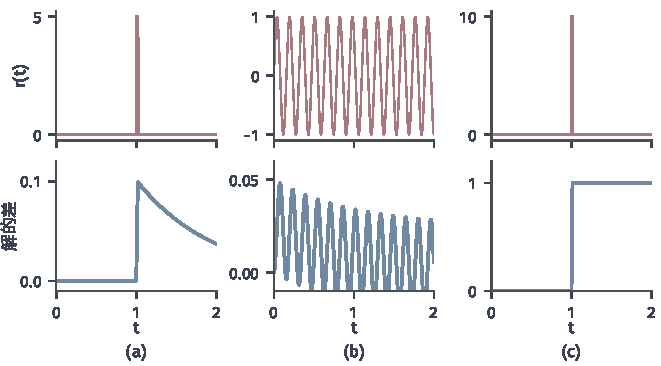
\includegraphics[width=112mm]{figures/06-differential-equations/01-ordinary-differential-equations/matplotlib/odesens-input-norms/figure.pdf}
  \caption{输入差的大小与解的差。上行是输入偏差$r(t)$，下行是解的差。(a)$\dot{x}=-x+g$，脉冲高$5$、宽$0.02$，积分$0.1$，解的差不超过$0.1$。(b)$\dot{x}=-x+g$，偏差$\sin40t$，积分范数约$1.27$，解的差却不超过$0.05$。(c)$\dot{x}=g^2$，脉冲高$10$、宽$0.01$，积分同为$0.1$，解的差却达到$1$。}
  \label{fig:odesens-input-norms}
\end{BookInlineFigure}

式~\eqref{eq:odesens-input-l1}是充分条件，不是必要条件。图~\ref{fig:odesens-input-norms}(b)的偏差$\sin40t$在$[0,2]$上的积分范数约为$1.27$，解的差却不超过$0.05$。原因是正负部分抵消，在加性输入下真正起作用的是偏差的累积$\int_{t_0}^{t}\bm{r}(s)\,\mathrm{d}s$，这里它不超过$2/40=0.05$。

非线性依赖就不同了。方程$\dot{x}=g^2$的残差是$\tilde{g}^2-g^2$，关于$g$的增长率随$\lvert g\rvert$变大。取$g\equiv0$，$\tilde{g}$是$[1,1+w)$上高度$A$的脉冲，
\[
 \int_0^2\lvert\tilde{g}-g\rvert\,\mathrm{d}t=Aw,\qquad y(2)-x(2)=A^2w.
\]
令$A=10$、$w=0.01$，输入差的积分只有$0.1$，解的差却是$1$，见图~\ref{fig:odesens-input-norms}(c)。让$A\to\infty$并保持$A^2w=1$，积分范数趋于零而解差不变。所以这里$L^1$小不足以保证解差小。

补救有两条路。若所有输入的值都限制在$\lVert\bm{g}\rVert_2\leq M$内，右端在这个范围内关于$\bm{g}$有常数$\ell=2M$，式~\eqref{eq:odesens-input-l1}恢复成立，$M$进入常数；上例$M=10$，$\ell\cdot Aw=20\times0.1=2$，确实不小于真实的$1$。另一条路是用更强的范数：一致范数$\sup_t\lVert\tilde{\bm{g}}-\bm{g}\rVert_2$小，就排除了高而窄的脉冲，只是它对孤立的短暂偏差过于敏感。

\paragraph{可测输入的条件}
上面的估计都只用到残差可积，没有用到输入的连续性。分段切换的输入、一般可测的输入都在其中，此时解是绝对连续函数，方程几乎处处成立。沿用第~\ref{chap:ode-existence-continuation}章的Carathéodory条件，右端沿解的复合是可测且局部可积的，式~\eqref{eq:odesens-residual}的$\varepsilon$因而有意义。但要得到定理~\ref{thm:odesens-basic-estimate}的结论，仍需要对时间可积的状态Lipschitz系数$L(t)$，这不是可测性能推出的。

\paragraph{方程的敏感性与求解器误差}
数值解也可以放进这个框架，这样能把两种常被混淆的误差分开。下面的计算只用定理的结构，数值方法本身放在第~\ref{chap:ode-numerical-methods}章。设网格$t_k=t_0+kh$，从$\bm{x}^{(0)}=\bm{x}_0$出发按
\[
 \bm{x}^{(k+1)}=\bm{x}^{(k)}+h\,\bm{f}(t_k,\bm{x}^{(k)})
\]
前进，把各点连成折线$\bm{y}(t)$。折线绝对连续，它的残差是$\bm{r}(s)=\dot{\bm{y}}(s)-\bm{f}(s,\bm{y}(s))$。

代入式~\eqref{eq:odesens-basic-estimate}，全局误差的上界是残差与放大因子乘积的积分。残差由求解器决定，步长越小残差越小。放大因子$\mathrm{e}^{\Lambda(t)-\Lambda(s)}$由方程决定，与求解器无关。前者是求解器的误差来源，后者是问题本身的敏感性。

\begin{example}[同一求解器，两个方程]
\label{ex:odesens-problem-solver}
取$\dot{x}=ax$，$x_0=1$，$h=1/4$，$T=1$，$a=\pm1$。在$[t_k,t_{k+1})$上，折线是$y(s)=x^{(k)}(1+a(s-t_k))$，于是
\[
 r(s)=\dot{y}-ay=-a^2x^{(k)}(s-t_k).
\]
方程线性，误差方程$\dot{e}=ae+r$可以精确求解，初值差为零时
\[
 y(1)-\mathrm{e}^{a}=\int_0^1\mathrm{e}^{a(1-s)}r(s)\,\mathrm{d}s.
\]

$a=1$时，$x^{(k)}$依次是$1,\,1.25,\,1.5625,\,1.9531,\,2.4414$；$a=-1$时依次是$1,\,0.75,\,0.5625,\,0.4219,\,0.3164$。逐段积分，得到
\[
 a=1:\ y(1)-\mathrm{e}=-0.2769,\qquad a=-1:\ y(1)-\mathrm{e}^{-1}=-0.0515.
\]
\end{example}

图~\ref{fig:odesens-problem-vs-solver}把三个量画在一起。两个方程的残差都是锯齿形，大小同为$h$的量级。权重却相反：$a=1$时早期残差被放大$\mathrm{e}^{1-s}>1$倍，$a=-1$时被缩小。误差相差五倍多，主要来自方程，而不是求解器。

\begin{BookInlineFigure}
  \centering
  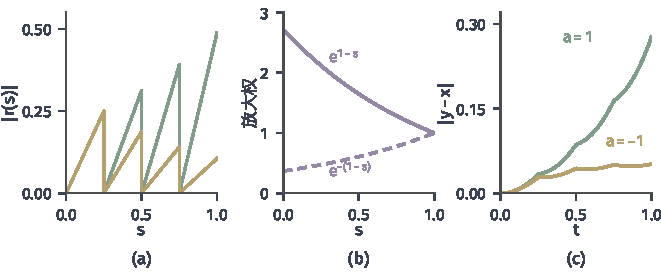
\includegraphics[width=112mm]{figures/06-differential-equations/01-ordinary-differential-equations/matplotlib/odesens-problem-vs-solver/figure.pdf}
  \caption{同一求解器在$\dot{x}=ax$上的表现，$h=1/4$，绿线$a=1$，黄线$a=-1$。(a)Euler折线的残差$\lvert r(s)\rvert$，由求解器决定。(b)放大权$\mathrm{e}^{a(1-s)}$，由方程决定（紫实线$a=1$，紫虚线$a=-1$）。(c)累积后的误差。}
  \label{fig:odesens-problem-vs-solver}
\end{BookInlineFigure}

因此，问题敏感时，再精细的求解器也只能把残差压小，放大因子还在；问题不敏感时，粗糙的残差也不至于造成大的全局误差。把解算准需要两者配合，这两者不可相互替代。
